\documentclass[8pt]{beamer}
\setbeamertemplate{navigation symbols}{}

\usepackage{graphicx}
\graphicspath{ {images/} }

\title{What is open source?}
\author{Brandon Moore}

\begin{document}

\begin{frame}
	\titlepage
\end{frame}

\section{Table of Contents}
\begin{frame}
	\frametitle{Table of Contents}
	\tableofcontents[]
\end{frame}

\section{What is open source?}
\begin{frame}
	\frametitle{Open Source Initiative definition}
	\begin{enumerate}
		\item \textbf{Free Redistribution} where the code can be changed or used in aggregate software and redistributed
		\item \textbf{Source Code} must be available ("the highest cost being a reasonable reproduction cost")
		\item \textbf{Derived Works} must be allowed at least under the same license
		\item \textbf{Integrity of the author's source code} can be maintained by enforcing modified versions to be released under a different name
		\item \textbf{No discrimination against any person or group of persons}
		\item \textbf{No discrimination against fields of endeavour} (politics, business, genetic engineering, etc)
		\item \textbf{Distribution of License} is maintained as the software is distributed
		\item \textbf{License must not be specific to a product} (aka I can take connman's dhcp code without the rest of it if I keep the license)
		\item \textbf{License must not restrict other software} by saying something like "I cannot be distributed alongside proprietary code"
		\item \textbf{License must be technology-neutral}
	\end{enumerate}
\end{frame}
\note{
	-Discuss the ambiguity brought on by OSI in 1998 chose "open source" terminology over "free software" (see Eric S. Raymond's 'Goodbye, "free software"; hello, "open source"' for more detail at http://www.catb.org/~esr/open-source.html). This ambiguity exists due to the slight differences between open source and free software although both hold a similar purpose.
	-Digress into how we don't hold open source to its truest meaning and will discuss things from hardware and creative commons to wireless security that isn't really open source.
	-We promote the creation of projects that adhere to the principles and spirit of open source and free software and promote learning and technical knowledge}

\section{Why Open source?}
\subsection{Security}
\begin{frame}
	\frametitle{Open Source is more secure}
	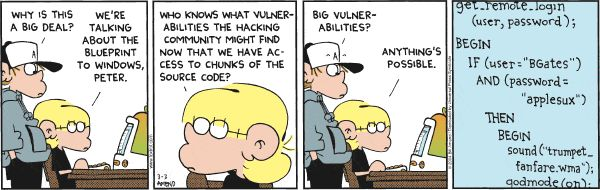
\includegraphics[width=\textwidth]{foxtrot_strip.jpg}
	\begin{itemize}
			\item \uncover<1->{People can audit the code for vulnerabilities}
			\item \uncover<2->{Backdoors are hard to hide}
			\item \uncover<3->{The security industry thrives on openness}
	\end{itemize}
\end{frame}

\begin{frame}
	
\includegraphics[scale=.8]{kalilinux.png}\\
	
\includegraphics[scale=.8]{openbsd.jpg}\centering\\
	
\includegraphics[scale=.6]{tox.png}\raggedleft
\end{frame}

\section{Who open sources?}
\begin{frame}
	\frametitle{Who open sources}
	Organizations devoted to open source:
	\begin{itemize}
		\item Mozilla
		\item Free Software Foundation (FSF is actually devoted to Free Software)
		\item Open Source Initiative (OSI)
		\item Apache Software Foundation
		\item Linux Foundation
		\item Many more
	\end{itemize}
	Where to find open source projects
	\begin{itemize}
		\item Github
		\item Bitbucket
		\item SourceForge
	\end{itemize}
\end{frame}

\section{Where is open source?}
\begin{frame}
	\begin{itemize}
		\item Have an Android? \begin{itemize}
				\item Android is open source
			\end{itemize}
		\item Have an Iphone or a Mac? \begin{itemize}
				\item The kernel (Darwin) is open source
			\end{itemize}
		\item TVs
		\item Routers
		\item Household appliances
		\item Web servers
	\end{itemize}
\end{frame}

\section{How to open source}
\begin{frame}
	\frametitle{How to contribute to open source (and why you should)}
	How to contribute-Making your own project\\
	\begin{itemize}
		\item Give your project a license
		\item Put it out there (Github, Bitbucket, GitLabs, etc)
	\end{itemize}
	How to contribute-Working on others' projects\\
	\begin{itemize}
		\item Find a project that enthuses you or something useful to you
		\item Start participating!
	\end{itemize}
\end{frame}

\begin{frame}
	\frametitle{But why should I?}
	\begin{itemize}
		\item Improve the tools you use everyday
		\item Improve your skills
		\item Build your resume!
	\end{itemize}
\end{frame}

\begin{frame}
	\frametitle{Questions?}
\end{frame}

\end{document}
